\section{Parameter Passing}

\section*{Where}
\begin{itemize}
  \item Register
  \item Global variables
  \item Stack
  \item Caller: PUSH parameter on stack
  \item Callee: Access parameter through LDR
\end{itemize}

\section*{Reentrancy}
\begin{itemize}
  \item Recursive Function Calls
  \item Registers and gobal variables are overwritten
  \item Requires an own set of data for each call
  \item Solution:
  \item ARM Procedure Call Standard
\end{itemize}

\section*{Passing through global variables}
\begin{itemize}
  \item Shared variables in data area
  \item Overhead to access variable
  \item Error prone, unmaintainable
  \item By reference
  \item Allows passing of larger structures
\end{itemize}

\section*{ARM Procedure call Standard}
\section*{Parameters}
\begin{itemize}
  \item Caller copies arguments From R0 to R3
  \item Caller copies additional parameters to stack
\end{itemize}

Returning fundamental data types

\begin{itemize}
  \item Smaller than word
  \item Word
  \item Double word
  \item 128-Bit\\
zero or sign extend to word return in RO return in RO / R1 return in RO - R3
\end{itemize}

Returning composite data types

\begin{itemize}
  \item Up to 4 bytes\\
return in RO
  \item Larger than 4 bytes stored in data area\\
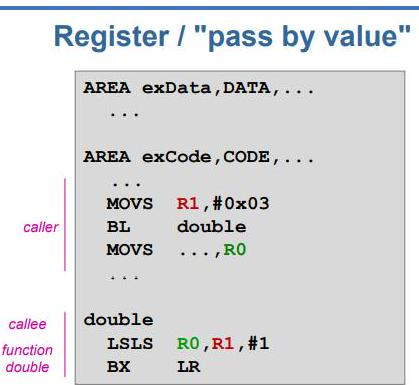
\includegraphics[width=\linewidth]{images/2024_12_29_79e6b22f503fb7b4f718g-09(2)}
\end{itemize}

Register Usage

\begin{center}
\begin{tabular}{|c|c|c|}
\hline
Register & Synonym & Role \\
\hline
ro & a1 & Argument / result / scratch register 1 \\
\hline
r1 & a2 & Argument / result / scratch register 2 \\
\hline
I2 & a3 & Argument / scratch register 3 \\
\hline
r3 & a4 & Argument / scratch register 4 \\
\hline
4$\tau$ & v1 & Variable register 1 \\
\hline
r5 & v2 & Variable register 2 \\
\hline
r6 & v3 & Variable register 3 \\
\hline
r7 & v4 & Variable register 4 \\
\hline
8$\tau$ & v5 & Variable register 5 \\
\hline
r9 & v6 & 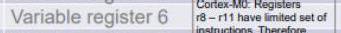
\includegraphics[width=\linewidth]{images/2024_12_29_79e6b22f503fb7b4f718g-09}
 \\
\hline
r10 & v7 & 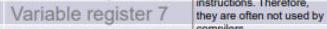
\includegraphics[width=\linewidth]{images/2024_12_29_79e6b22f503fb7b4f718g-09(1)}
 \\
\hline
r11 & v8 & Variable register 8 \\
\hline
r12 & IP & Intra-Procedure-call scratch register1) \\
\hline
r13 & SP &  \\
\hline
r14 & LR &  \\
\hline
\end{tabular}
\end{center}

Register contents\\
might be modified\\
might be modified

Callee must preserve contents\\
of these registers (Callee saved)\\
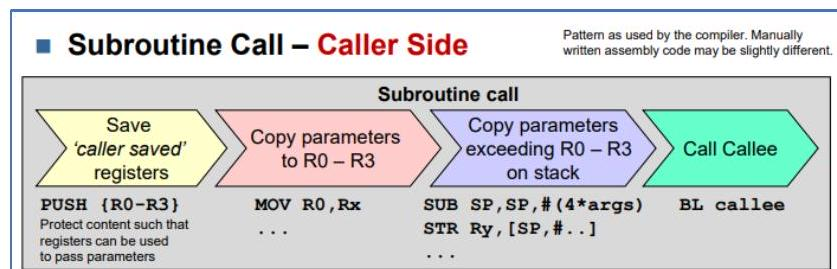
\includegraphics[width=\linewidth]{images/2024_12_29_79e6b22f503fb7b4f718g-09(3)}

On return from subroutine